% タイトル
\chapter{線の形}
\vspace{-45pt} %高さ調整
\begin{flushright}
  {\bf \large 理工学部 物理科学科 2回生} \\ \vspace{3pt} %所属
  {\bf \large 中山 敦貴} \\ \vspace{30pt} %名前
\end{flushright}


%
\section*{はじめに}
去年の会誌ではサインカーブとカテナリー曲線の話をした。今回もそれの続きとしてまた曲線の話である。メインは最速降下曲線の話であるが、これは去年の会誌でやるつもりだったが、なかなか手強くて今回リベンジすることになった。ついでにインボリュート曲線とトラクトリックスという曲線についても考えた。これらについてはただ計算をガリガリしたかっただけである。

%%%%%%%%%%%%%%%%%%%%%%%%%%%%%%%%%%%%%%%%%%%%%%%%%%%%
\section{インボリュート曲線}
%%%%%%%%%%%%%%%%%%%%%%%%%%%%%%%%%%%%%%%%%%%%%%%%%%%%

\subsection{インボリュート曲線とは}
\begin{wrapfigure}{r}{40mm}
  \centering
  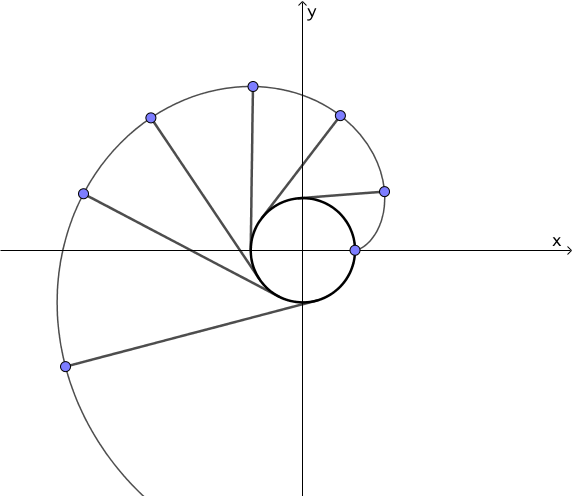
\includegraphics[width = 6cm]{nakayama1/image/imbo3}
\end{wrapfigure}
円形の筒に糸が巻かれている。その糸をピンと張りながらほどいていくとき、糸の端点が描く軌道をインボリュート曲線と呼ぶ。

\subsection{曲線の式}
それでは早速、この曲線の式を求めてみよう。半径$a$の円筒に糸が巻きつけられているとして、その糸をピンと張りながらどんどんほどいていくときを考える。

\begin{figure}[H]
  \centering
  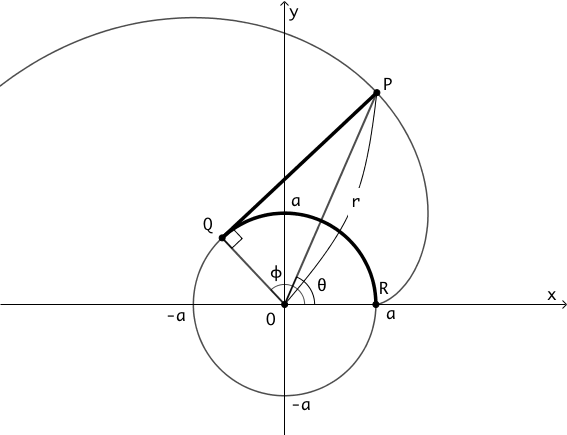
\includegraphics[width=8cm]{nakayama1/image/imbo1}
\end{figure}

円弧$\ko{QR}$の長さは、ほどいた糸$\mathrm{PQ}$の長さに等しいので
\begin{align*}
  \ko{QR} = 2\pi a \times \frac{\phi}{2\pi} = a\phi = \mathrm{PQ}
\end{align*}
となる。
よって$\triangle \mathrm{OPQ}$で次のことが言える。
\begin{spacing}{0.2}
\end{spacing}
  \begin{align*}
    \sin(\phi - \theta) &= \frac{a\phi}{r} \qquad\qquad \text{$\mathrm{PQ} = a\phi$だから}\\
    \sin\phi \cos\theta - \cos\phi \sin\theta &= \frac{a\phi}{r} \qquad\qquad \text{左辺を加法定理でバラした}\\
    r\cos\theta \sin\phi - r\sin\theta \cos\phi &= a\phi \qquad\qquad \text{両辺に$r$をかけた}\\
    x\sin\phi - y\cos\phi &= a\phi \qquad\qquad \text{直交座標に直した}
  \end{align*}
また、同様にして
\begin{spacing}{1}
  \begin{align*}
    \cos(\phi - \theta) &= \frac{a}{r}\\
    \cos\phi \cos\theta + \sin\phi \sin\theta &= \frac{a}{r} \qquad\qquad \text{左辺を加法定理でバラした}\\
    r\cos\theta \cos\phi + r\sin\theta \sin\phi &= a \qquad\qquad \text{両辺に$r$をかけた}\\
    x\cos\phi + y\sin\phi &= a \qquad\qquad \text{直交座標に直した}
  \end{align*}
\end{spacing}\noindent
よって、$x$と$y$についての式が2つ得られた
\begin{align*}
  \begin{cases}
  \,\cos\phi \cos\theta + \sin\phi \sin\theta = \dfrac{a}{r}\\
  \,x\cos\phi + y\sin\phi = a
  \end{cases}
\end{align*}
あとはこの連立方程式を解けばいいのだが、せっかくなので線形代数の力を借りて美しく解いてみようと思う。\par
まずは2式を行列を使って表す。
\begin{align*}
  \begin{pmatrix}
    \sin\phi & -\cos\phi \\
    \cos\phi & \sin\phi \\
  \end{pmatrix}
  \begin{pmatrix}
    x\\y\\
  \end{pmatrix}
  =
  \begin{pmatrix}
    a\phi\\a\\
  \end{pmatrix}
\end{align*}
行列式を計算すると
\begin{align*}
  \begin{vmatrix}
    \sin\phi & -\cos\phi \\
    \cos\phi & \sin\phi \\
  \end{vmatrix}
  =\sin^2\phi + \cos^2\phi = 1
\end{align*}
であるから、クラーメルの公式より
  \begin{align*}
    x &=
    \begin{vmatrix}
      a\phi & -\cos\phi \\
      a & \sin\phi \\
    \end{vmatrix}
    = a(\cos\phi + \phi\sin\phi)\\
    y &=
    \begin{vmatrix}
      \sin\phi & a\phi \\
      \cos\phi & a \\
    \end{vmatrix}
    = a(\sin\phi - \phi\cos\phi)
  \end{align*}
よってインボリュート曲線は
\begin{align*}
  \begin{cases}
  \,x = a(\cos\phi + \phi\sin\phi)\\
  \,y = a(\sin\phi - \phi\cos\phi)
  \end{cases}
\end{align*}
とパラメータ表示できることがわかった。

\begin{figure}[H]
  \centering
  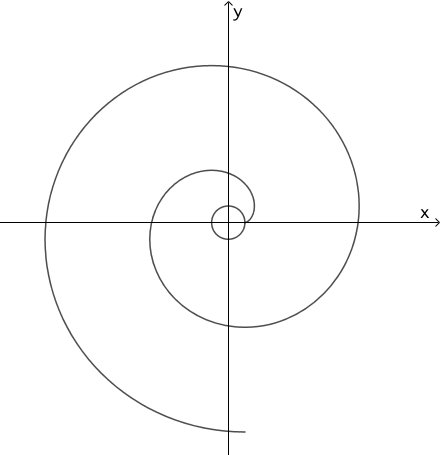
\includegraphics[width=8cm]{nakayama1/image/imbo2}\\
  $0 \le \phi \le 4\pi$におけるインボリュート曲線
\end{figure}

\subsection{伸開線}
  一般に、ある曲線に巻きつけられた糸を弛まないように引っ張りつつほどいていくときの、糸の端点が描く軌道を伸開線という。円の伸開線はさっき求めたインボリュート曲線である。前回の会誌で考えたカテナリー曲線の伸開線は、次節で紹介するトラクトリックスになっている。暇な人は考えてみよう。伸開線のWikipediaにわかりやすいGIFがあるので見てみるとよい。


%%%%%%%%%%%%%%%%%%%%%%%%%%%%%%%%%%%%%%%%%%%%%%%%%%%%
\section{トラクトリックス}
%%%%%%%%%%%%%%%%%%%%%%%%%%%%%%%%%%%%%%%%%%%%%%%%%%%%

\subsection{トラクトリックスとは}
石ころに紐を結び、図のように$x$軸に沿って紐を引くとき、石ころが描く軌道をトラクトリックスまたは牽引曲線と呼ぶ。
また、各点での接線と$x$軸との間の長さが一定であるような曲線であるとも言える。\par
\begin{figure}[H]
  \centering
  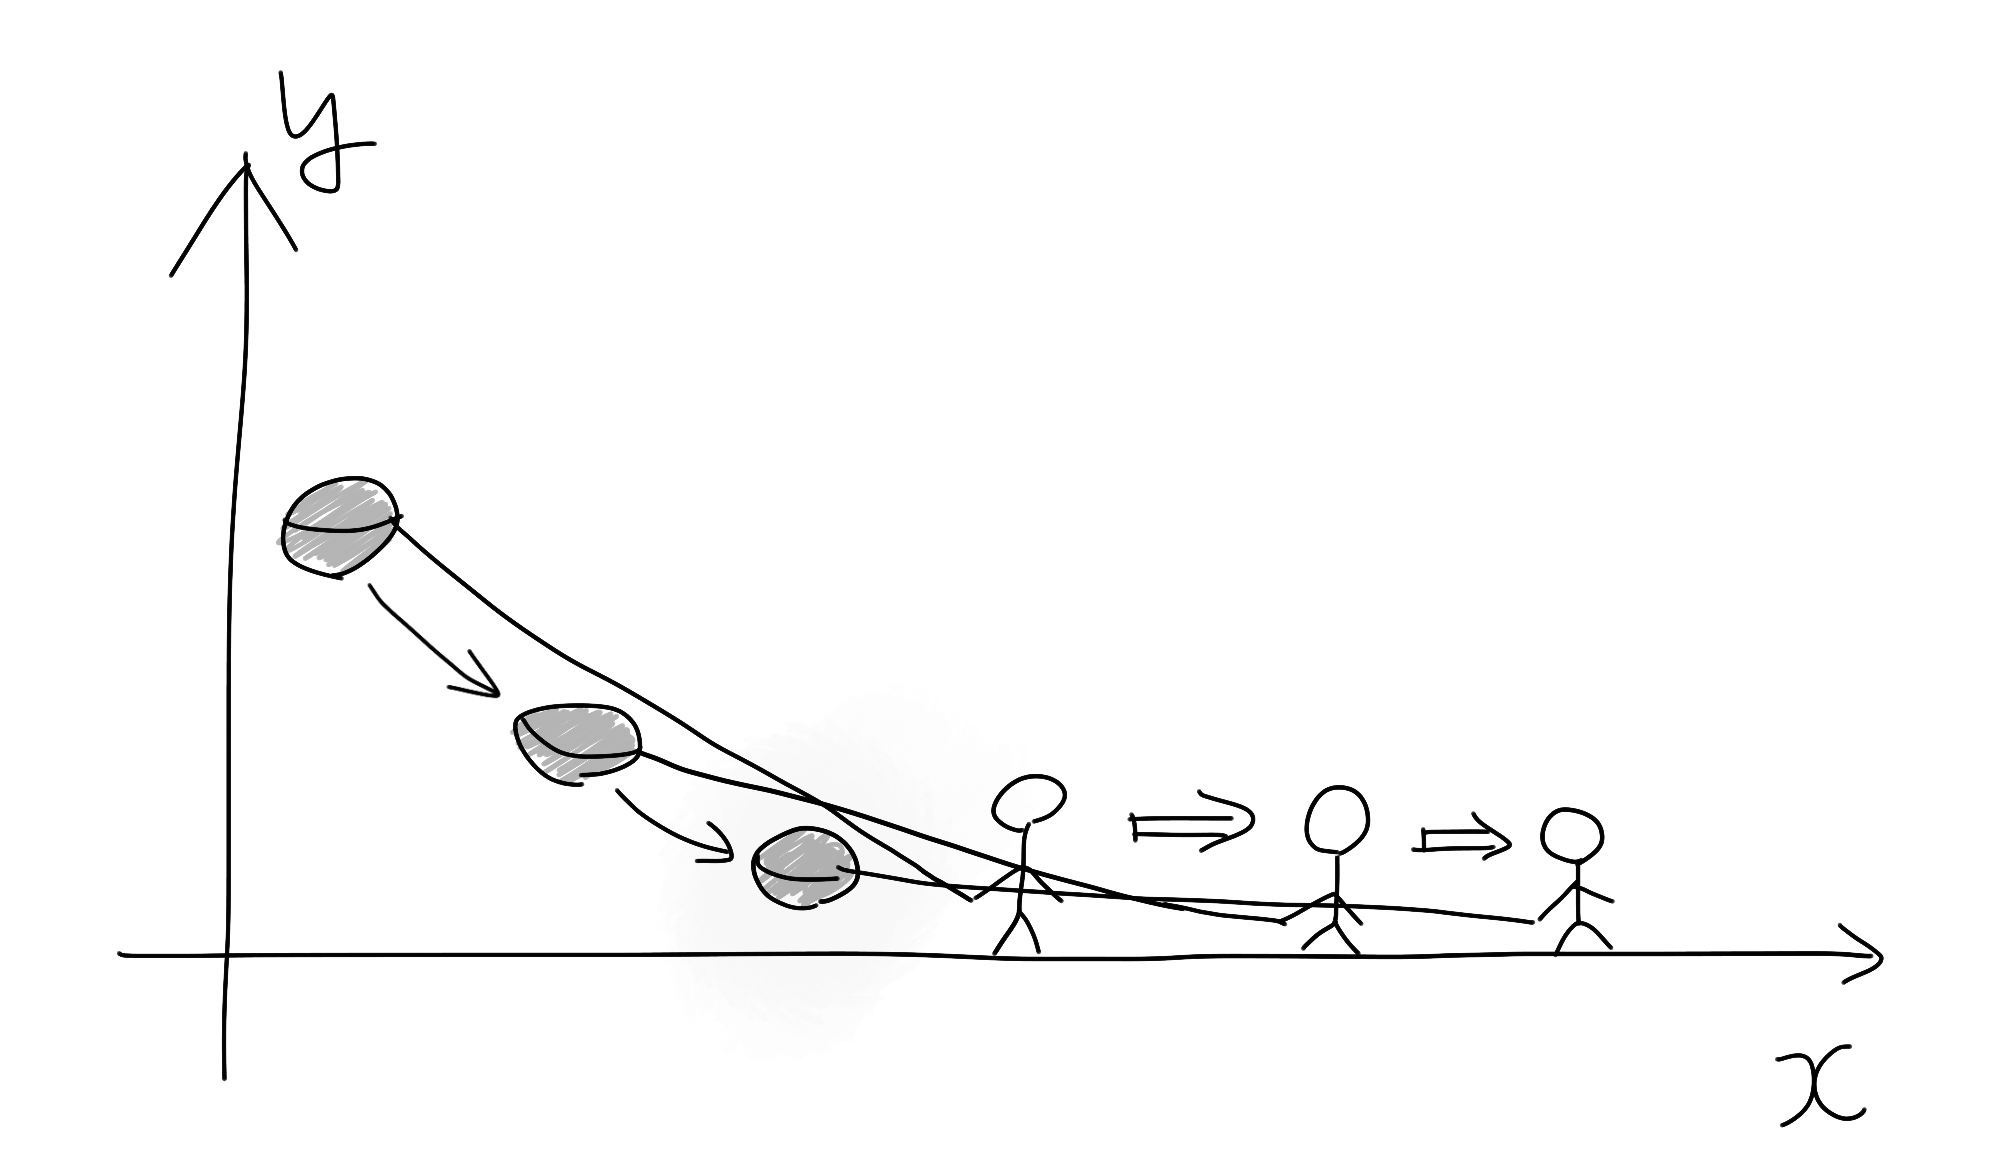
\includegraphics[width=8cm]{nakayama1/image/trac1}\\
  {\small トラクトリックスが描かれていく様子}
\end{figure}

\subsection{曲線の式}

初めの石ころの位置を$(0,a)$、引っ張る人の位置を原点$(0,0)$とする。ここから引っ張る人は$x$軸上を右に進んでいく。\par
石ころに力を伝えるのは紐であるから、紐は常に作用線上にある。作用線は曲線の導関数に一致するので、紐は接線上にあることになる。

\begin{figure}[H]
  \centering
  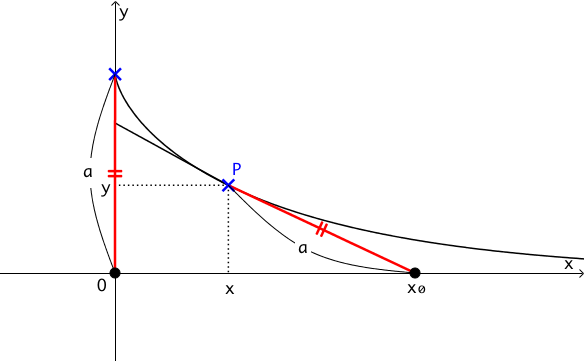
\includegraphics[width=8cm]{nakayama1/image/trac2}
\end{figure}

三平方の定理より
\begin{align*}
  y^2 + (x_0 - x)^2 &= a^2 \\
  (x_0 - x)^2 &= a^2 - y^2
\end{align*}
$x < x_0$であるから
\begin{align*}
  x_0 - x &= \sqrt{a^2 - y^2}
\end{align*}
よって、接線の傾きを考えると
\begin{align*}
  \frac{\mathrm{d}y}{\mathrm{d}x} = - \frac{y}{x_0 - x} = - \frac{y}{\sqrt{a^2 - y^2}}
\end{align*}
が成り立つことがわかる。あとはこの微分方程式を$x$について解いていく。\par
まずは変数を分離して両辺積分する。
\begin{align*}
  \mathrm{d}x &= - \frac{\sqrt{a^2 - y^2}}{y} \,\mathrm{d}y \\
  \int \mathrm{d}x &= - \int \frac{\sqrt{a^2 - y^2}}{y} \,\mathrm{d}y \\
  x &= - \int \frac{\sqrt{a^2 - y^2}}{y} \,\mathrm{d}y
\end{align*}
右辺は置換積分で計算する。$u = \sqrt{a^2 - y^2}$とおくと、$0 < y$であるから
\begin{align*}
  y = \sqrt{a^2 - u^2}
\end{align*}
よって
\begin{align*}
  \frac{\mathrm{d}y}{\mathrm{d}u} = - \frac{u}{\sqrt{a^2 - u^2}}
\end{align*}
であるから、これらで置換して
\begin{align*}
  x &= - \int \frac{u}{\sqrt{a^2 - u^2}} \cdot \left(- \frac{u}{\sqrt{a^2 - u^2}}\right) \,\mathrm{d}u \\
  &= \int \frac{u^2}{a^2 - u^2} \,\,\mathrm{d}u
\end{align*}
少し変形すると
\begin{align*}
  x &= - \int \frac{u^2}{u^2 - a^2} \,\,\mathrm{d}u \\
  &= - \int \frac{u^2 - a^2 + a^2}{u^2 - a^2} \,\,\mathrm{d}u \\
  &= - \int\mathrm{d}u - \int \frac{a^2}{u^2 - a^2} \,\,\mathrm{d}u \\
  &= - u - \int \frac{a^2}{u^2 - a^2} \,\,\mathrm{d}u
\end{align*}
ここで第2項の被積分関数を
\begin{align*}
  \frac{a^2}{u^2 - a^2} = \frac{A}{u - a} + \frac{B}{u + a}
\end{align*}
の形に部分分数分解できると仮定して$A,B$を求める。
分母を払って
\begin{align*}
  a^2 &= A(u + a) + B(u - a)\\
  &= (A + B)u + aA - aB
\end{align*}
両辺の$u$の係数を比較して
\begin{align*}
  \begin{cases}
    A + B = 0\\
    aA - aB = a^2
  \end{cases}
\end{align*}
これを解くと
\begin{spacing}{0.5}
  \begin{align*}
    \begin{cases}
      \,A = \dfrac{a}{2} \cr\cr
      \,B = - \dfrac{a}{2}
    \end{cases}
  \end{align*}
\end{spacing}\noindent
となるので
\begin{align*}
  \frac{a^2}{u^2 - a^2} &= \frac{a}{2}\cdot\frac{1}{u - a} - \frac{a}{2}\cdot\frac{1}{u + a}
\end{align*}
と部分分数分解できる。よって
\begin{align*}
  x &= - u - \int \frac{a^2}{u^2 - a^2} \,\,\mathrm{d}u \\
  &= - u - \frac{a}{2} \int \frac{\mathrm{d}u}{u - a} + \frac{a}{2} \int \frac{\mathrm{d}u}{u + a} \\
  &= - u - \frac{a}{2} \log{|u - a|} + \frac{a}{2}\log{|u + a|} + C \\
  &= - u - \frac{a}{2} \log{\left| \frac{u - a}{u + a} \right|} + C \\
  &= - \sqrt{a^2 - y^2} - \frac{a}{2} \log{\left| \frac{\sqrt{a^2 - y^2} - a}{\sqrt{a^2 - y^2} + a} \right|} + C
\end{align*}
$0 < y \leq a$であることに注意して絶対値を外すと
\begin{align*}
  x &= - \sqrt{a^2 - y^2} - \frac{a}{2} \log{\frac{a - \sqrt{a^2 - y^2}}{a + \sqrt{a^2 - y^2}}} + C
\end{align*}
となる。積分定数$C$は、$x = 0$のとき$y = a$という初期条件より
$$ C = 0$$
であることがわかる。\par
よってこの場合のトラクトリックスは
\begin{align*}
  x &= - \frac{a}{2} \log{\frac{a - \sqrt{a^2 - y^2}}{a + \sqrt{a^2 - y^2}}} - \sqrt{a^2 - y^2}\\
  &= - \frac{a}{2} \log{\frac{y^2}{(a + \sqrt{a^2 - y^2})^2}} - \sqrt{a^2 - y^2}\\
  &= a\log{\frac{a + \sqrt{a^2 - y^2}}{y}} - \sqrt{a^2 - y^2}
\end{align*}
で表すことができる。

%%%%%%%%%%%%%%%%%%%%%%%%%%%%%%%%%%%%%%%%%%%%%%%%%%%%
\section{最速降下曲線}
%%%%%%%%%%%%%%%%%%%%%%%%%%%%%%%%%%%%%%%%%%%%%%%%%%%%

\subsection{最速降下曲線とは}
坂道の高いところにある地点Aから低いところにある地点Bまでボールを転がす\footnote{滑らすと言った方が正確。あとで地点Aでの位置エネルギーが地点Bで運動エネルギーにのみ変換されたということを使うため。ボールが転がると、回転にエネルギーを取られてしまう。}。このとき、坂道の地点Aから地点Bまでボールが転がるのにかかる時間が最小になるような坂の形を最速降下曲線と呼ぶ。\par
地点AからBまでを結ぶ距離が最短となる一直線の坂が一番速いように思えるが、実はそうではない。いろいろな形の坂を作って実験してみてほしい。

\subsection{ボールが転がる時間}
\begin{wrapfigure}{r}{50mm}
  \centering
  \vspace{-5zw}
  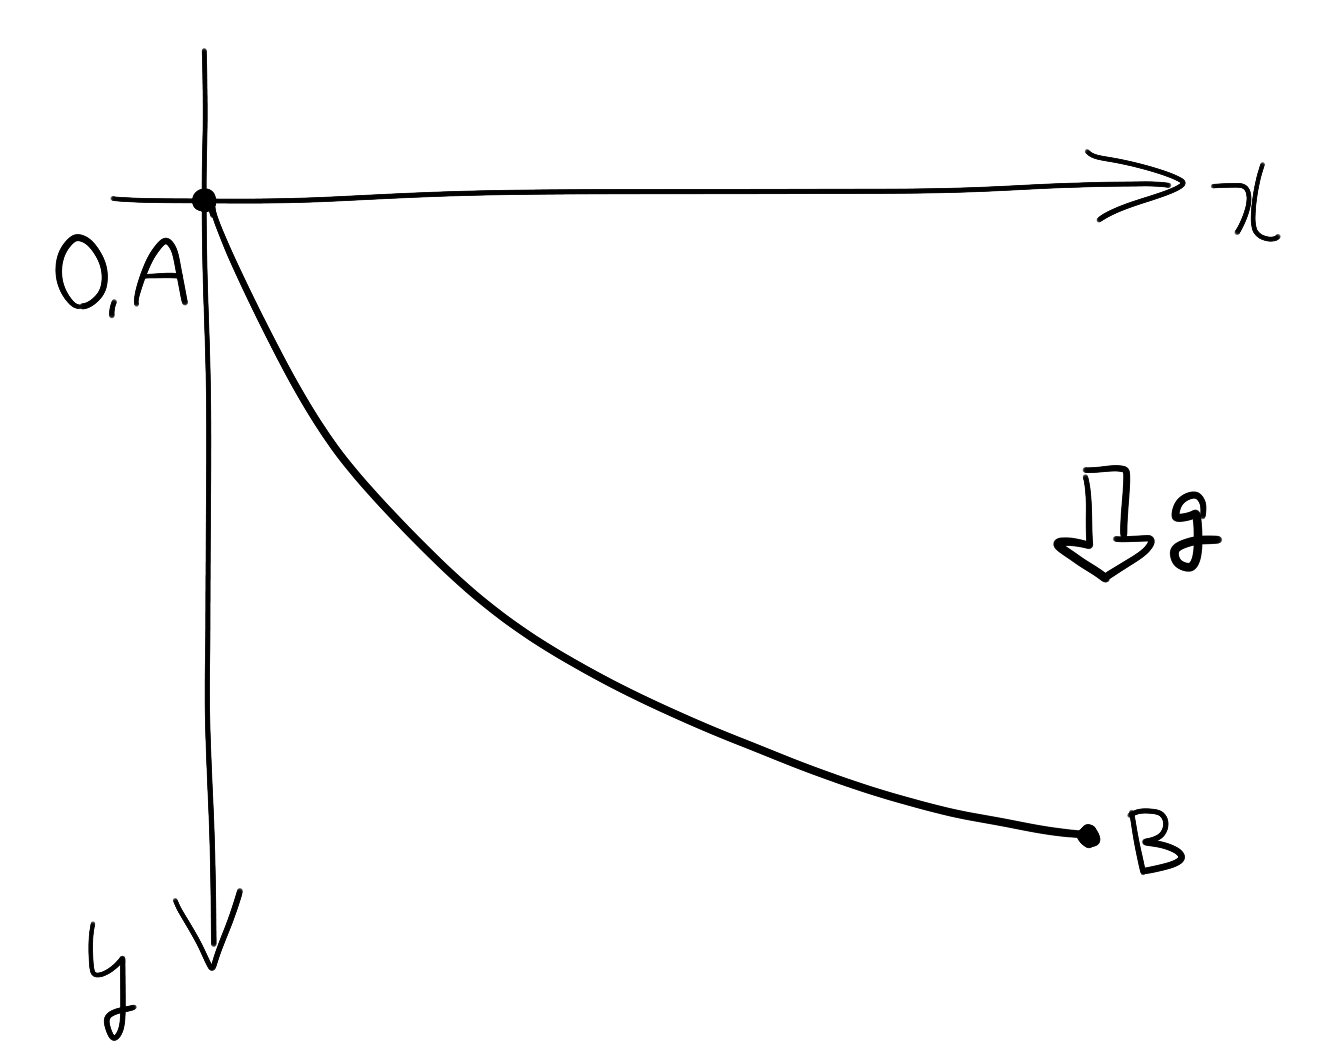
\includegraphics[width = 5cm]{nakayama1/image/zahyou}
\end{wrapfigure}
この曲線の式を求めるために、まずは坂道の地点Aから地点Bまでボールが転がるのにかかる時間を式で表そう。まずは図のように座標をとる。地点Aを原点Oとする。また、$y$軸を下向きにとっているので注意。


ボールの微小変位$\dd L$は三平方の定理より
\begin{align*}
  \dd L = \sqrt{\dd x^2 + \dd y^2}
        = \sqrt{1 + \left( \frac{\dd y}{\dd x} \right)^2} \,\,\dd x
\end{align*}\par
ボールの速度を$v$、重力加速度を$g$とすれば、力学的エネルギー保存則より
\begin{align*}
  v = \sqrt{2gy}
\end{align*}
であるから、ボールが$\dd L$だけ転がるのにかかる微小時間$\dd t$は
\begin{align*}
  \dd t = \frac{\dd L}{v} = \sqrt{\frac{1 + (y')^2}{2gy}} \,\,\dd x
\end{align*}\par
よって求める時間はこれを積分して
\begin{align*}
  T = \int_A^B \dd t = \int_A^B \sqrt{\frac{1 + (y')^2}{2gy}} \,\,\dd x
\end{align*}
と表すことができる。\par
今知りたいのはこの$T$を最小にするような$y$の形である。しかし、それを考えるには変分法という新しい技を身につけなければならない。\par
次節では変分法について簡単に解説し、必要な公式を導出する。

\subsection{変分法}

\subsubsection{変分法とは}
微分を勉強した時に、$y = f(x)$が最小値をとるときの$x$の値を求める問題を考えたことがあると思う。もし端点以外に$y$が最小値をとるときがあるとすれば、$y$はそこで極値をとる。つまり$y$の導関数$y'$が$y' = 0$となるときの$x$を調べれば$y$が最小値をとる可能性のある$x$を見つけることができる(極大値をとるかもしれないが)。\par
今回の問題もこの方法で解決できそうだが、少し勝手が違う。先ほど求めた$T$は積分された形にはなっているが、$y$の関数となっている。しかしその$y$は$x$の関数となっている。つまり$T$は関数の関数という形になっている。今回の$T$のように、関数を変数にとるような関数は汎関数と呼ばれている。\par
微分法が関数について研究するところであるとすると、変分法は汎関数について研究するところであると言える。

\subsubsection{汎関数$F(y)$の極値}

ここでは$T$を少し一般化した
$$ F(y) := \int_a^b f(x,y(x),y'(x)) \,\dd x$$
で定義された$F(y)$について考える。知りたいのはこの$F(y)$が極値をとるときの$y$の形である。\par
そこで以下のように、$y$の形を少し変えたものとして$y_\epsilon$を定義する。
$$ y_\epsilon (x) := y(x) + \epsilon h(x) $$
ただし、$h(x)$は$h(a) = h(b) = 0$を満たす任意の関数\footnote{端点は固定するという意味。坂道の話でいうとスタート地点とゴール地点は変えないということ。}、$\epsilon$は任意の実数であるとする。このように定義された$y_\epsilon$を$y$の$h$方向の変分という。\par
そうすると、$y_\epsilon$は$\epsilon$の関数であるから、$F(y_\epsilon)$も$\epsilon$の関数となる。\par
\begin{figure}[H]
  \centering
  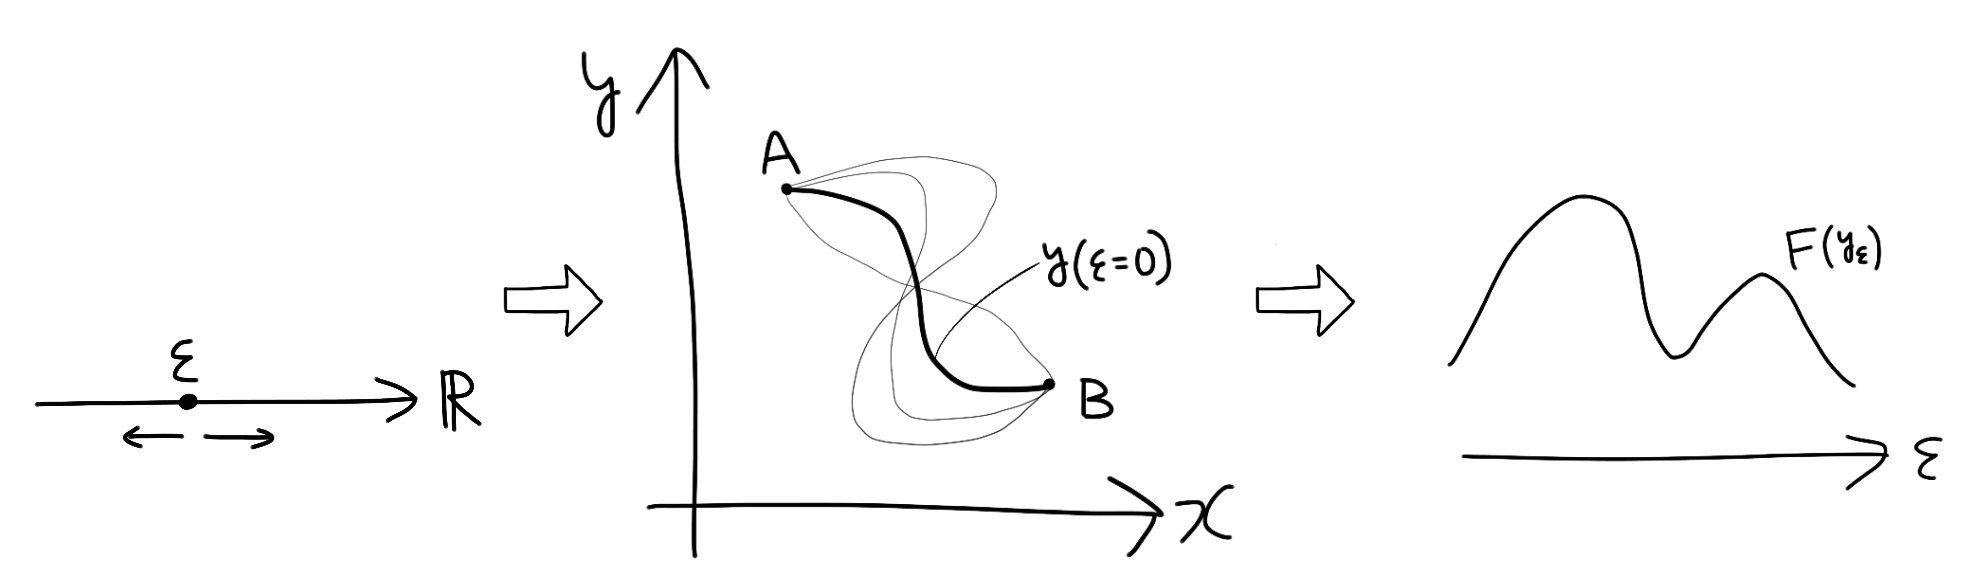
\includegraphics[width = 100mm]{nakayama1/image/henbun.png}\\
  {\small 変分原理のイメージ図}
\end{figure}

$F(y_\epsilon)$が$\epsilon$の関数ならば、$F(y_\epsilon)$は$\epsilon$で微分可能である。つまり微分法のときと同じように考えて$\dfrac{\dd F(y_\epsilon)}{\dd \epsilon} = 0$のとき$F(y_\epsilon)$は極値をとることがわかる。
よって$\dfrac{\dd F(y_\epsilon)}{\dd \epsilon} = 0$とおけば、$F(y_\epsilon)$が極値をとるときの$\epsilon$の値がわかる。$\epsilon$の値がわかれば、それから$y_\epsilon$がわかる。つまりその$y_\epsilon$に対して$F(y_\epsilon)$は極値をとる。
以上のことから、もし$y_\epsilon = y$($\epsilon = 0$のとき)で$F(y_\epsilon)$が極値をとるなら
$$\left. \dfrac{\dd}{\dd \epsilon}F(y_\epsilon) \right|_{\epsilon = 0} = 0$$
が成り立つ。つまりこれを満たす$y_\epsilon$($=y$)が$F$が極値をとるときの関数となっている。また
$$\delta F := \left. \dfrac{\dd}{\dd \epsilon}F(y_\epsilon) \right|_{\epsilon = 0}$$
で定義される$\delta F$を汎関数$F$の第一変分といい、$\delta F = 0$を満たす点$y$を$F$の臨界点または停留点という。\par
以上が変分法についての簡単な(?)説明である。最後に微分法と変分法の対応を書いておく。

\begin{table}[H]
  \begin{center}
    {\gt \small 微分法と変分法の対応}\\
    \begin{tabular}{cc}
      微分 & 変分\\ \hline
      関数$f$ & 汎関数$F$\\
      関数$f$の微分$f'=0$ & 汎関数$F$の変分$\delta F=0$\\
      関数$f$が極値をとる点$x$ & 汎関数$F$の臨界点$y$
    \end{tabular}
  \end{center}
\end{table}

\subsubsection{オイラー=ラグランジュの方程式}

前節では$F(y_\epsilon)$が極値となるような$y_\epsilon$が知りたければ、汎関数$F$の第一変分$\delta F = 0$を満たす$y_\epsilon$を見つければよいということがわかった。この節では$\delta F = 0$を計算して、オイラー=ラグランジュの方程式を導く。\par
まずは$F(y)$の定義を思い出す。
$$ F(y) = \int_a^b f(x,y(x),y'(x)) \,\dd x$$
よって$F$の第一変分は
\begin{align*}
  \delta F
  = \left. \dfrac{\dd}{\dd \epsilon}F(y_\epsilon) \right|_{\epsilon = 0}
  &= \left. \frac{\dd}{\dd \epsilon} \int_a^b f(x,y_\epsilon (x),y'_\epsilon (x)) \,\dd x \right|_{\epsilon = 0} \\
  &= \left. \int_a^b \frac{\dd f}{\dd \epsilon} \,\dd x \right|_{\epsilon = 0}
\end{align*}
合成関数の微分法より
\begin{align*}
  \hspace{43mm} &= \left. \int_a^b \left( \frac{\partial f}{\partial y_\epsilon} \cdot \frac{\dd y_\epsilon}{\dd \epsilon} + \frac{\partial f}{\partial y_\epsilon'} \cdot \frac{\dd y_\epsilon'}{\dd \epsilon} \right) \dd x \right|_{\epsilon = 0} \\
  &= \left. \int_a^b \left( \frac{\partial f}{\partial y_\epsilon} \cdot \frac{\dd y_\epsilon}{\dd \epsilon} + \frac{\partial f}{\partial y_\epsilon'} \cdot \frac{\dd}{\dd x} \frac{\dd y_\epsilon}{\dd \epsilon} \right)\dd x \right|_{\epsilon = 0} \\
  &= \left. \int_a^b \left( \frac{\partial f}{\partial y_\epsilon} \cdot h(x) + \uwave{\frac{\partial f}{\partial y_\epsilon'} \cdot \frac{\dd}{\dd x}h(x)} \right)\dd x \right|_{\epsilon = 0}
\end{align*}
ここで\uwave{第2項}を部分積分すると
\begin{align*}
  \int_a^b \frac{\partial f}{\partial y_\epsilon'} \cdot \frac{\dd}{\dd x}h(x) \,\dd x
  &= \left[ \frac{\partial f}{\partial y_\epsilon'} \cdot h(x) \right]_a^b - \int_a^b \frac{\dd}{\dd x}\frac{\partial f}{\partial y_\epsilon'} \cdot h(x) \,\dd x
\end{align*}
$h(a) = h(b) = 0$より
$$\left[ \frac{\partial f}{\partial y_\epsilon'} \cdot h(x) \right]_a^b = 0$$
となるので
\begin{align*}
  \int_a^b \frac{\partial f}{\partial y_\epsilon'} \cdot \frac{\dd}{\dd x}h(x) \,\dd x
  &= - \int_a^b \frac{\dd}{\dd x}\frac{\partial f}{\partial y_\epsilon'} \cdot h(x) \,\dd x
\end{align*}
元の式に戻して
\begin{align*}
  \delta F &= \left. \int_a^b \left( \frac{\partial f}{\partial y_\epsilon} - \frac{\dd}{\dd x}\frac{\partial f}{\partial y_\epsilon'} \right)h(x) \,\dd x \right|_{\epsilon = 0} \\
  &= \int_a^b \left( \frac{\partial f}{\partial y} - \frac{\dd}{\dd x}\frac{\partial f}{\partial y'} \right)h(x) \,\dd x
\end{align*}
よって$F$が極値をもつ条件は
\begin{align*}
  \int_a^b \left( \frac{\partial f}{\partial y} - \frac{\dd}{\dd x}\frac{\partial f}{\partial y'} \right)h(x) \,\dd x = 0
\end{align*}
が成り立つことである。$h(x)$は任意関数であるから、これが常に成り立つとすると
\begin{align*}
  \frac{\partial f}{\partial y} - \frac{\dd}{\dd x}\frac{\partial f}{\partial y'} = 0
\end{align*}
という方程式が得られる。これをオイラー=ラグランジュの方程式と呼ぶ。\par
あとはこの方程式に$f = T = \sqrt{\dfrac{1 + (y')^2}{2gy}}$を代入して解けばいいのだが、計算が大変になるので、もう少しこの方程式を変形しよう。

\subsubsection{ベルトラミの公式}
前節でオイラー=ラグランジュの方程式を導出したときは$f = f(x,y,y')$としていたが、今回考えたい$T$は$x$を陽に(直接には)含んでいないので、オイラー=ラグランジュの方程式はもう少し簡単な形に変形することができる。$f = f(y,y')$としてもう少し考えよう。\par
$f$の全微分は
$$\dd f(y,y') = \frac{\partial f}{\partial y}\dd y + \frac{\partial f}{\partial y'}\dd y'$$
であるから、両辺$\dd x$で割って
\begin{align*}
  \frac{\dd f}{\dd x} &= \frac{\partial f}{\partial y} \frac{\dd y}{\dd x} + \frac{\partial f}{\partial y'} \frac{\dd y'}{\dd x} \\
  &= \uwave{y'\frac{\partial f}{\partial y}} + \frac{\dd y'}{\dd x} \frac{\partial f}{\partial y'}
\end{align*}\par
一方、オイラー=ラグランジュの方程式の両辺に$y'$をかけると
$$0 = y'\left( \frac{\partial f}{\partial y} - \frac{\dd}{\dd x}\frac{\partial f}{\partial y'} \right)
= \uwave{y'\frac{\partial f}{\partial y}} - y'\frac{\dd}{\dd x}\frac{\partial f}{\partial y'}$$\par
この2式から$\uwave{y'\dfrac{\partial f}{\partial y}}$を消去すると
\begin{align*}
  \frac{\dd f}{\dd x} &= \frac{\dd y'}{\dd x} \frac{\partial f}{\partial y'} + y'\frac{\dd}{\dd x}\frac{\partial f}{\partial y'} \\
  &= \frac{\dd}{\dd x} \left( y'\frac{\partial f}{\partial y'} \right)
\end{align*}\par
両辺$x$で積分して
\begin{align*}
  \int \frac{\dd f}{\dd x} \,\dd x &= \int \frac{\dd}{\dd x} \left( y'\frac{\partial f}{\partial y'} \right) \dd x \\
  f &= y'\frac{\partial f}{\partial y'} + C
\end{align*}\par
よって
\begin{align*}
  \qquad\qquad f - y'\frac{\partial f}{\partial y'} = C \qquad\quad\text{($C$は任意定数)}
\end{align*}\par
という方程式が得られる。これをベルトラミの公式と呼ぶ。

\subsection{最速降下曲線の形}
変分法の話が長くなったが、あとはベルトラミの公式から$T$が極値をとるときの$y$(これが知りたかったもの)がわかるので、$f = T$を代入して計算してみよう。
\begin{align*}
  C &= T - y'\frac{\partial T}{\partial y'} \\
  &= \sqrt{\frac{1 + (y')^2}{2gy}} - y'\frac{\partial}{\partial y'} \sqrt{\frac{1 + (y')^2}{2gy}} \\
  &= \sqrt{\frac{1 + (y')^2}{2gy}} - \frac{y'}{\sqrt{2gy}} \frac{\partial}{\partial y'} \sqrt{1 + (y')^2} \\
  &= \sqrt{\frac{1 + (y')^2}{2gy}} - \frac{y'}{\sqrt{2gy}} \frac{y'}{\sqrt{1 + (y')^2}} \\
  &= \frac{1 + (y')^2 - (y')^2}{\sqrt{2gy\{1 + (y')^2\}}} \\
  &= \frac{1}{\sqrt{2gy\{1 + (y')^2\}}}
\end{align*}\par
よって
$$\sqrt{2gy\{1 + (y')^2\}} = \frac{1}{C}$$\par
両辺2乗して
\begin{align*}
  2gy\{1 + (y')^2\} &= \frac{1}{C^2} \\
  y\{1 + (y')^2\} &= \frac{1}{2gC^2}
\end{align*}\par
定数を$2r \equiv \frac{1}{2gC^2}$と置き直して
\begin{align*}
  y\{1 + (y')^2\} &= 2r \\
  (y')^2 &= \frac{2r}{y} - 1
\end{align*}
ここで両辺ルートをとるが、坂道なので$y' > 0$のときだけ考える。
\begin{align*}
  \frac{\dd y}{\dd x} \equiv y' &= \sqrt{\frac{2r}{y} - 1} \\
  &= \frac{\sqrt{2ry - y^2}}{y} \\
  &= \frac{\sqrt{r^2 - (r^2 - 2ry + y^2)}}{y} \\
  &= \frac{ \sqrt{r^2 - (r - y)^2} }{y}
\end{align*}
よって
\begin{align*}
  \dd x & = \frac{y}{ \sqrt{r^2 - (r - y)^2} }\,\dd y
\end{align*}
両辺積分すると
\begin{align*}
  x = \int \frac{y}{ \sqrt{r^2 - (r - y)^2} }\,\dd y
\end{align*}
$y = r(1 - \cos\theta)$とおくと、$\dd y = r\sin\theta \,\dd \theta$であるから
\begin{align*}
  x &= \int \frac{r(1 - \cos\theta)}{r \sqrt{1 - \cos^2 \theta}}\,r\sin\theta\,\dd \theta \\
  &= \int r(1 - \cos\theta)\,\dd \theta \\
  &= r(\theta - \sin\theta) + \mathrm{const.}
\end{align*}
原点を通るとして、$x = 0$のとき$y = 0$。またこのとき$\theta = 0$であるから$\mathrm{const.} = 0$。よって
\begin{align*}
  \begin{cases}
    \, x = r(\theta - \sin\theta)\\
    \, y = r(1 - \cos\theta)
  \end{cases}
\end{align*}
と媒介変数表示できた。これはサイクロイドである。

\begin{figure}[H]
  \centering
  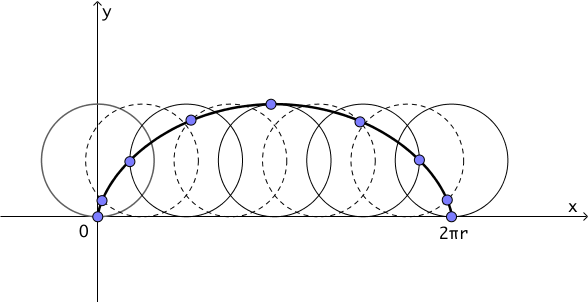
\includegraphics[width=8cm]{nakayama1/image/cyco}\\
  {\small サイクロイドの図。円を転がすとき、円周に固定した点が描く軌道がサイクロイド。\\
  今回の話では$y$軸を下向きを正としていたことに注意。つまりこれを上下反転したものになる。}
\end{figure}

%
\clearpage
\section*{参考文献}
\begin{enumerate}
  \item[] \hspace{-20pt}{\gt インボリュート曲線}
  \item インボリュート曲線 - Wikipedia,「\url{https://ja.wikipedia.org/wiki/インボリュート曲線}」
  \item 伸開線 - Wikipedia,「\url{https://ja.wikipedia.org/wiki/伸開線}」
  \item[] \hspace{-20pt}{\gt トラクトリックス}
  \item トラクトリックス - Wikipedia, 「\url{https://ja.wikipedia.org/wiki/トラクトリックス}」
  \item Tractrix.pdf,「\url{http://izumi-math.jp/M_Matumoto/Tractrix.pdf}」
  \item[] \hspace{-20pt}{\gt 変分法}
  \item 変分法 - Wikipwdia,「\url{https://ja.wikipedia.org/wiki/変分法}」
  \item 変分法1 [物理のかぎしっぽ], 「\texttt{http://hooktail.sub.jp/mathInPhys/variations1/}」
  \item @minami106, 変分法の入門編, 「\texttt{http://minami106.web.fc2.com/math/henbun2.pdf}」
    \item 西山豊, 最速降下問題,
    「\url{http://www.osaka-ue.ac.jp/zemi/nishiyama/math2010j/cycloid_j.pdf}」
  \item 山上滋, 微積分II,\\
  「\url{https://www.math.nagoya-u.ac.jp/~yamagami/teaching/calculus/cal2011akib.pdf}」
\end{enumerate}





%
